\documentclass{beamer}

\usepackage[sfdefault]{cabin}
\usepackage[utf8]{inputenc}
\usepackage[T1]{fontenc}
\usepackage[french]{babel}
\usepackage{xcolor}
\usepackage{caption}
\usepackage{graphicx}
%Police
%\usepackage[sfdefault]{roboto}
\usepackage[sfdefault]{FiraSans}

%\definecolor{modernblue}{RGB}{100, 152, 204} 
\definecolor{modernvert}{RGB}{0, 80, 0} 

\usetheme{Boadilla}

\usecolortheme[named=modernvert]{structure}

\setbeamertemplate{caption}{\insertcaption} % Utiliser le format de légende par défaut de beamer

\renewcommand{\thesection}{\Roman{section}}\renewcommand{\thesubsection}{\arabic{subsection} }\renewcommand{\thesubsubsection}{\alph{subsubsection} }

\newcommand{\C}{\mathbb{C}}\newcommand{\R}{\mathbb{R}}\newcommand{\Q}{\mathbb{Q}}\newcommand{\Z}{\mathbb{Z}}\newcommand{\N}{\mathbb{N}}\newcommand{\V}{\overrightarrow}\newcommand{\Cs}{\mathscr{C}}\newcommand{\Ps}{\mathscr{P}}\newcommand{\Rs}{\mathscr{R}}\newcommand{\Gs}{\mathscr{G}}\newcommand{\Ds}{\mathscr{D}}\newcommand{\happy}{\huge\smiley}\newcommand{\sad}{\huge\frownie}\newcommand{\alors}{\Large\Rightarrow}\newcommand{\equi}{\Leftrightarrow}
\newcommand{\disp}{\displaystyle}\newcommand{\Pro}{\mathbb{P}}


\newtheorem{thm}{Théorème}
\newtheorem{rmq}{Remarque}
\newtheorem{prop}{Propriété}
\newtheorem{cor}{Corollaire}
\newtheorem{lem}{Lemme}
\newtheorem{prop-def}{Propriété-définition}

\theoremstyle{definition}

\newtheorem{defi}{Définition}
\newtheorem{intro}{Initialisation}
\newtheorem{boucle}{Boucle principale}
\newtheorem{ex}{Exemple}
\newtheorem*{rap}{Rappel}
\newtheorem{cex}{Contre-exemple}
\newtheorem{exer}{Exercice} % \large {\fontfamily{ptm}\selectfont EXERCICE}
\newtheorem{nota}{Notation}
\newtheorem{ax}{Axiome}
\newtheorem{appl}{Application}
\newtheorem{csq}{Conséquence}
\def\di{\displaystyle}


\title{Transport optimal et distances de Wasserstein}
\author{Tudal Crequy et Ivanhoé Botcazou}
\date{27 mai 2023}
\begin{document}
\begin{frame}[plain]
    \maketitle
\end{frame}

\section{Introduction}
\begin{frame}
	
\frametitle{Introduction}

	\begin{minipage}[t]{1\linewidth}
	\begin{minipage}{0.4\linewidth}\centering\begin{figure}
			\centering
			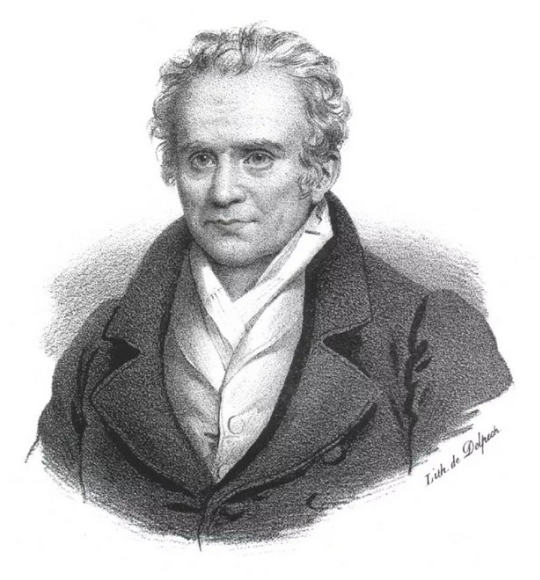
\includegraphics[scale=0.25]{monge.png}
			\caption*{Gaspard Monge (1746-1818)}
		\end{figure}\end{minipage}\quad \quad 
	\begin{minipage}{0.43\linewidth}\centering\begin{figure}
			
			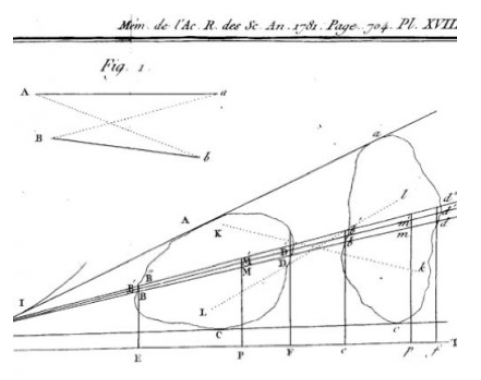
\includegraphics[scale=0.35]{sable.png}			
			\caption*{Extrait de la théorie des déblais et des remblais}
		\end{figure}\end{minipage}
	\end{minipage}
\end{frame}

\begin{frame}
	
	\frametitle{}
	\begin{minipage}[t]{1\linewidth}
	\begin{minipage}{0.4\linewidth}\centering\begin{figure}
			\centering
			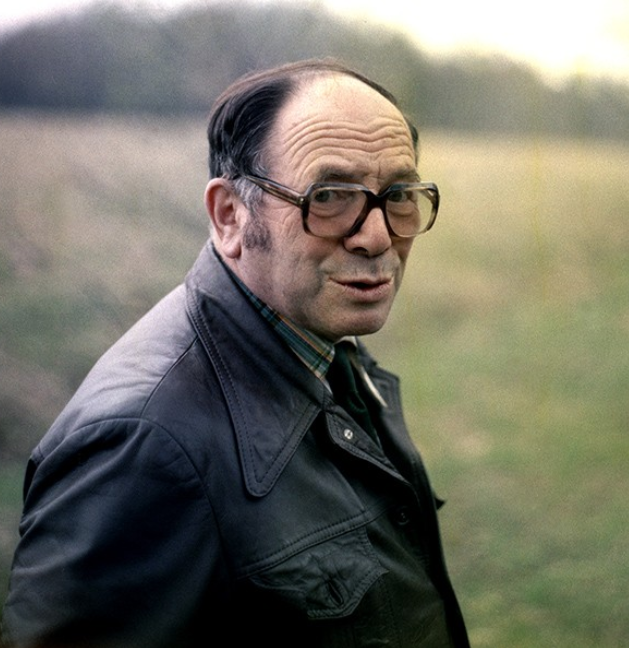
\includegraphics[scale=0.25]{Kantorovich.png}
			\caption*{ Leonid Vitalievitch Kantorovitch (1912-1986)}
	\end{figure}\end{minipage}\hfil
	\begin{minipage}{0.43\linewidth}\centering\begin{figure}
			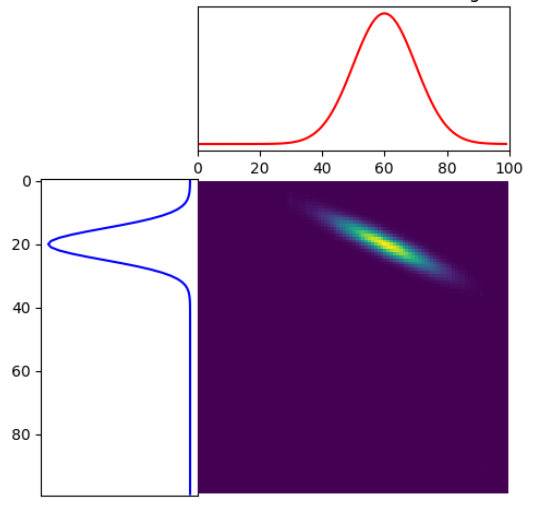
\includegraphics[scale=0.3]{couplage.png}			
			\caption*{Mesure de couplage}
	\end{figure}\end{minipage}
\end{minipage}
\end{frame}

\begin{frame}
	\tableofcontents
\end{frame}


\section{Formulation du problème}
\subsection{Modélisation du problème par Monge}

\begin{frame}
	\frametitle{Modélisation du problème par Monge}\hfill\\[-0.8cm]
			\begin{figure}
			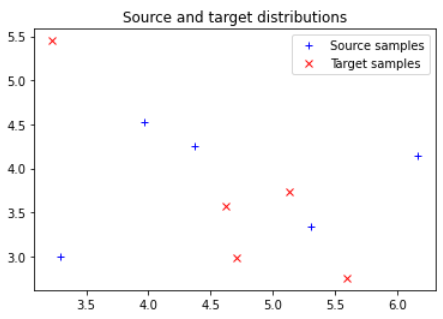
\includegraphics[scale=0.42]{a2.png}	\hfill\\[-0.8cm]			
		\end{figure}
	\begin{itemize}
		\item Soit $\displaystyle\mu = \sum_{i=1}^{n}\alpha_i\delta_{\{x_i\}}$ une mesure de probabilité source. 
		\item Soit $\displaystyle \nu = \sum_{i=1}^{m}\beta_i\delta_{\{y_i\}}$ une mesure de probabilité cible.
		\item $\underline{But} :$ Construire une application $T : \R^2 \to \R^2$ transportant $\mu$ sur $\nu$ sous une certaine contrainte et avec un coût minimal. 
	\end{itemize}

\end{frame}

\begin{frame}
	%\frametitle{Modélisation du problème par Monge}%\hfill\\[-2cm]
	\begin{itemize}
		\item $\underline{\text{La contrainte sur T}}$ :\\
		 la \emph{mesure image} de $\mu$ par $T$ est égale à $\nu$. 
			$$ T_{\#\mu}(\cdot) = \mu(T^{-1}(\cdot)) = \nu(\cdot)$$
		\item $\underline{\text{Le coût d'un transporteur}}$ :  
	\end{itemize}\begin{itemize}
	\item[$\bullet$] Une fonction de coût peut être la distance induite\\
	 par la norme euclidienne $\|\cdot\|$ sur $\R^2$ par exemple.
	\item[$\bullet$] Le coût d'un transporteur du plan $T_1$ est donné par:
	
	$$C(T_1) = \int_{\R^2}\|x -T_1 (x)\| \ \mu(dx).$$
	Dans le cas discret :
	$$C(T_1) = \sum_{i=1}^{n}\|x_i -T_1 (x_i)\| \times \alpha_i.$$ 
	
	\item $\underline{\text{Transporteur optimal}}$ :\\
	$T^*$ une application réalisant l'infimum:
	$$T^* = \text{arginf}\{C(T ); \ T : \R^2 \to \R^2 , \ T_{\#\mu} = \nu\}$$
\end{itemize}
	
\end{frame}

\begin{frame}
	\frametitle{Les limites du problème de Monge}
	\begin{minipage}[t]{1\linewidth}
		\begin{minipage}{0.4\linewidth}\centering\begin{figure}
				\centering
				\includegraphics[scale=0.27]{carrés.png}
				\caption{ Non unicité du transport optimal. Translation ou symétrie, certainement pas une rotation.}
		\end{figure}\end{minipage}\hfil\quad \quad \quad \quad
		\begin{minipage}{0.43\linewidth}\centering\begin{figure}
				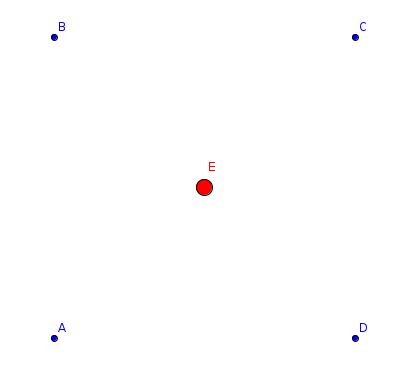
\includegraphics[scale=0.35]{points.png}			
				\caption{Transport à sens unique}
		\end{figure}\end{minipage}
	\end{minipage}
\end{frame}

\subsection{Assouplissement des contraintes, problème de Monge-Kantorovich}

\begin{frame}
	\frametitle{Assouplissement des contraintes, problème de Monge-Kantorovich}
		\begin{minipage}[t]{1\linewidth}
	\begin{minipage}{0.44\linewidth}\centering\begin{figure}
			\begin{itemize}
				\item Une vision probabiliste et non déterministe du problème. 
				\item Soit $\mu,\nu\in \mathcal P(\R)$ et $(X,Y)$ un couple de variables aléatoires de loi marginale respective $\mu,\nu$. On note $\pi\in\mathcal P(\R\times\R)$ la loi du couple. 
				\item $\Pi(\mu, \nu)$ l'ensemble des couplages possibles.   
			\end{itemize}
	\end{figure}\end{minipage}\hfil
	\begin{minipage}{0.43\linewidth}\centering\begin{figure}
			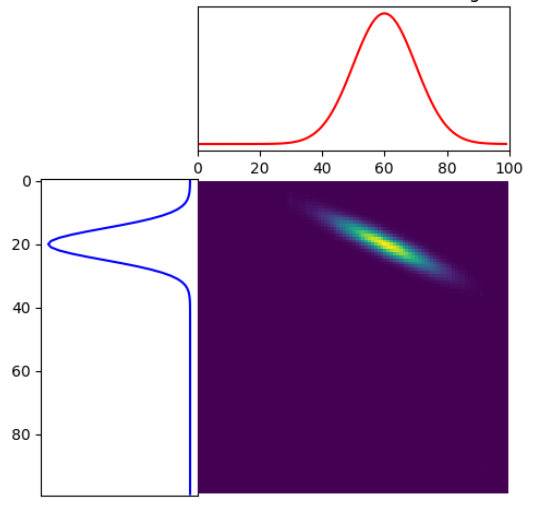
\includegraphics[scale=0.3]{couplage.png}			
			\caption{Mesure de couplage $\pi$}
	\end{figure}\end{minipage}
\end{minipage}
\end{frame}

\begin{frame}
		\begin{itemize}
				\item Un transport est donné par un couplage $\pi$. Pour $c$ une fonction de coût on obtient le coût du transport:
				$$I_c (\pi) = \iint_{\R\times\R }
				c(x, y) \pi(dxdy)$$
				\item Problème de Monge-Kantorovich $\alors$ optimisation sur l'espace des couplages possibles. 
				\item Si le minimum est réalisé, $I_c (\pi^*) = T_c (\mu, \nu)$, on dit que $\pi^*$ est un couplage optimal.
				 $$\mathcal T_c (\mu, \nu) = \text{inf }\big\{I_c (\pi) \ : \ \pi \in \Pi(\mu, \nu) \big\}$$
				  $$\pi^* = \text{argmin }\big\{I_c (\pi) \ : \ \pi \in \Pi(\mu, \nu) \big\}$$
			\end{itemize}

\end{frame}

\section{Existence d'une solution, dualité de Kantorovich et distance de Wasserstein}
\subsection{Existence d'un plan de transport optimal}

\begin{frame}
	\frametitle{Existence d'un plan optimal}
	\begin{defi}
		\begin{minipage}[t]{1\linewidth}
			\begin{minipage}{0.55\linewidth}
				Une fonction $f : E \to \R \cup\{+\infty\}$ est dite semi-continue inférieurement en $x \in E$	si pour toute suite $(x_n)_{n\in\N}$ convergeant vers $x$, on a
				$$\lim\limits_{n\to +\infty}\inf f (x_n ) \geq f(x)$$
			\end{minipage}\hfill
			\begin{minipage}{0.47\linewidth}
				$$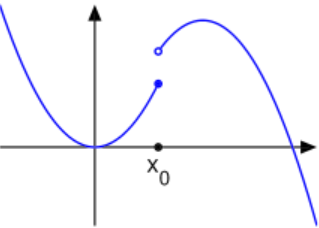
\includegraphics[scale=0.35]{sci.png}$$
			\end{minipage}
		\end{minipage}	
	\end{defi}
\begin{thm}
	Soit $c : E \times E \to [0, +\infty]$ une fonction de coût $sci$. Pour toutes mesures de probabilité $\mu, \nu \in \mathcal P(E )$, il existe $\pi^*\in\Pi(\mu,\nu)$ tel que
	
	$$I_c (\pi^*) = \iint_{E \ E }
	c(x, y) \pi^*(dxdy) = T_c (\mu, \nu) = \text{inf }\big\{I_c (\pi) \ : \ \pi \in \Pi(\mu, \nu) \big\}$$\end{thm}
 
\end{frame}


\subsection{Distances de Wasserstein}
\begin{frame}
	\frametitle{Introduction à la distance de Wasserstein}
	\begin{defi}
		Pour  $p \in [1, +\infty[$ on pose $\mathcal P_p(E )$ l'ensemble des mesures de probabilité qui admettent un moment d'ordre $p$.
		
		%$$\mathcal P_p(E ) = \left\{ \mu \in \mathcal P(E ) : \exists x_0 \in E, \int_{E }d(x,x_0)^pd\mu(x) < +\infty \right\}$$
	\end{defi}
	\begin{prop-def}
		Pour tout couple $(\mu,\nu)\in \mathcal P_p(E )^2$, la quantité 
		$$W_p(\mu,\nu) = T_p (\mu, \nu)^{\frac{1}{p}} $$
		\noindent est appelée la distance de Wasserstein suivant la valeur $p$. L'application $$\begin{array}{cccl}W_p :& \mathcal P_p(E )^2&  \longrightarrow& \R^+\\
		&(\mu,\nu)&\longmapsto&T_p (\mu, \nu)^{\frac{1}{p}}
		\end{array}$$ 
		\noindent est une distance sur $\mathcal P_p(E )$.
	\end{prop-def}
\end{frame}

\subsection{Dualité de Kantorovich}
\begin{frame}
	\frametitle{Dualité de Kantorovich}
	\begin{thm}
		Soit $c : E \times E \to [0, +\infty[$ une fonction de coût $sci$. Pour toutes mesures de probabilité $\mu, \nu \in \mathcal P(E )$ telles que $T_c (\mu, \nu) < +\infty$. On a alors
		$$T_c (\mu, \nu) = \sup\limits_{(\varphi,\psi)\in \Phi_b^2}\left\{\int_{E}\varphi(x)d\mu(x) + \int_{E}\psi(y)d\nu(y)\right\} $$
		\noindent où $\Phi_b$ est l'ensemble des fonctions continues bornées telles que
		$$\psi(x) + \varphi(y) \leq c(x, y), \quad \forall x, y \in E.$$
	\end{thm} 
\end{frame}


\section{Algorithmes et applications}

\subsection{Algorithmes Hongrois}

\begin{frame}
	\frametitle{Présentation de l'algorithme Hongrois}
	\begin{defi}
		 \textbf{Linear Sum Assignment Problem (LSAP)} est un cas particulier du problème discret. Les mesures $\mu$ et $\nu$ ont le même nombre $N$ de points, et les $p_i$ et $q_i$ sont égaux à $\frac{1}{N}$.\\[0.25cm]
		\noindent$\bullet$ La matrice de couplage a une contrainte supplémentaire :\\ les $x_{ij}$ sont égaux à 0 ou 1.
	\end{defi}
L'approche "duale" permet de faciliter la recherche de solutions:
\begin{prop}
	L'algorithme Hongrois permet de construire une assignation optimale pour le problème de LSAP relâché. On construit un couple faisable solution du problème dual ($\phi$, $\psi$) tel que $\phi(i) + \psi(j) \leq c_{ij}$
\end{prop} 
\end{frame}

\begin{frame}
	L'assignation vide $x = 0_n$ et ($\phi$, $\psi$) nulles. On « augmente » d'abord $\phi$ et $\psi$ en deux étapes. \\
	L'arête $(i,j)$ est saturée si $\phi(i)+\psi(j)=c_{i,j}$.
			\begin{minipage}[t]{1\linewidth}
		\begin{minipage}{0.48\linewidth}
			\begin{intro}
				\begin{itemize}
					\item Pour $1\leq i\leq n$: $\phi(i) = \underset{j}{min}(c_{ij})$.
					\item Puis $1\leq j\leq n$: $\psi(j) = \underset{i}{min}(c_{ij} - \phi(i))$.
					\item Pour $1\leq i\leq n$:
					\begin{itemize}
						\item[$\bullet$] S'il existe $j$ non-assigné avec l'arête $(i, j)$ saturée, on assigne $i$ au premier $j$ trouvé ( $x_{ij}=1$) 
						\item[$\bullet$] Sinon i reste non-assigné.
					\end{itemize}
										
					  
				\end{itemize}
			\end{intro}
		\end{minipage}\hfill
		\begin{minipage}{0.47\linewidth}
				\begin{boucle}
					Pour chaque sommet non assigné :
				\begin{itemize}
					\item Chercher un chemin augmentant dans le graphe des arêtes saturées. 
					\begin{itemize}
						\item[$\bullet$] S'il y en a un, l'inverser.
						\item[$\bullet$] S'il n'y en a pas, créer des arêtes saturées en modifiant ($\phi$, $\psi$), et revenir au 1. C'est la procédure d'\textbf{ouverture d'arêtes saturées}.
					\end{itemize}  
				\end{itemize}
			\end{boucle}
		\end{minipage}
	\end{minipage}	 
\end{frame}

%\begin{frame}\centering 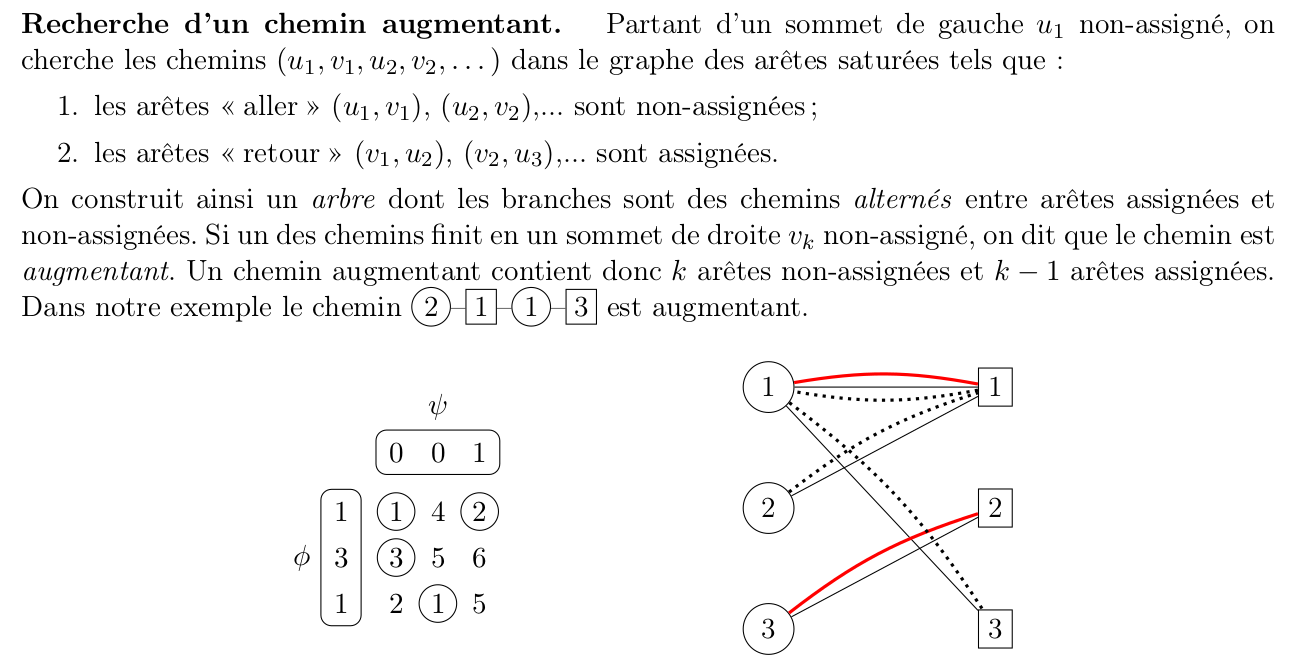
\includegraphics[scale=0.26]{chemin_augmentant.png}\end{frame}

\begin{frame}$$c= \begin{pmatrix}	7&9&8&9\\	2&8&5&7\\	1&6&6&9\\	3&6&2&2	\end{pmatrix}$$
\centering 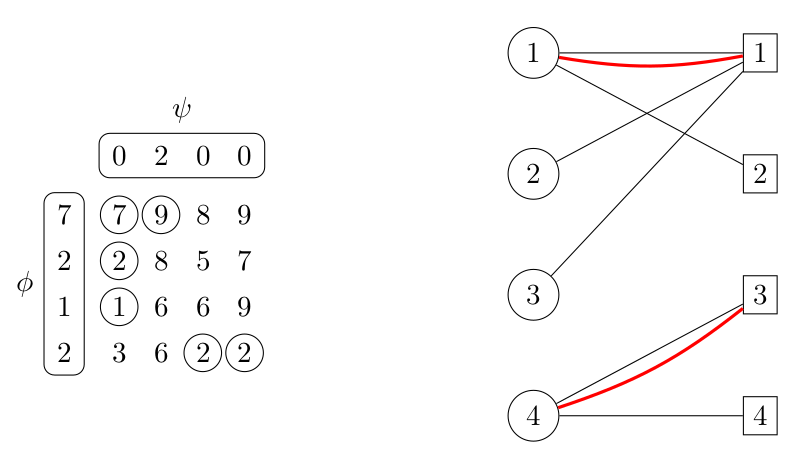
\includegraphics[scale=0.3]{z1.png}
\end{frame}
\begin{frame}
	\centering 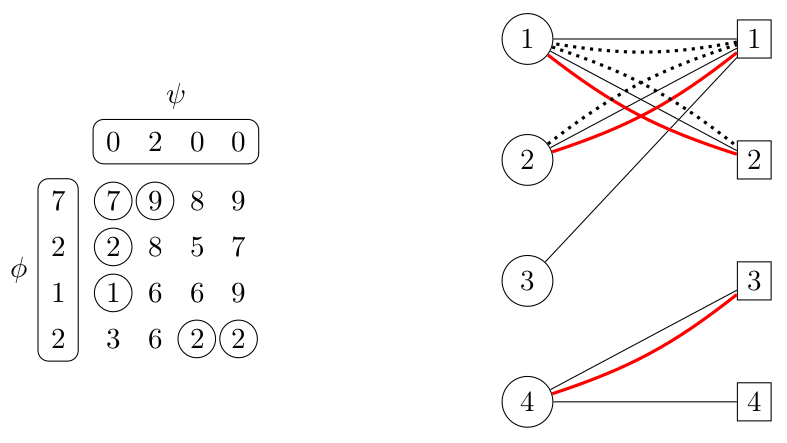
\includegraphics[scale=0.35]{z2.png}
	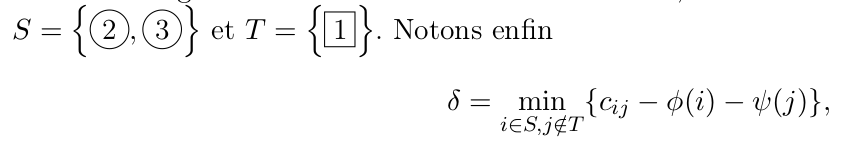
\includegraphics[scale=0.3]{z4.png}
\end{frame}


\begin{frame}
	\begin{minipage}{0.45\linewidth}
		$$i= 2 \quad \left\{\begin{array}{l} 8-2-2 = 4 \quad j= 2\\
		\textbf{5 - 2 - 0 = 3 \quad\quad j=3 }\\
		7-2-0 =5 \quad j= 4\end{array}
		\right.$$
	\end{minipage}\hfil
\begin{minipage}{0.45\linewidth}
	$$i= 3 \quad \left\{\begin{array}{l} \textbf{6-5-2 = 3 \quad\quad\quad j= 2}\\
	6 - 1 - 0 = 5 \quad j=3 \\
	9-1-0 =8 \quad j= 4\end{array}
	\right.$$
\end{minipage}
\centering
	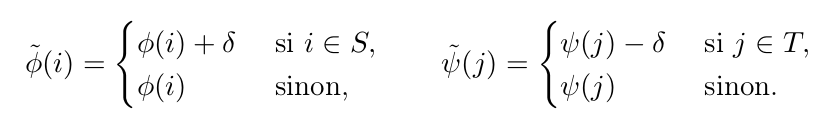
\includegraphics[scale=0.35]{z5.png}
	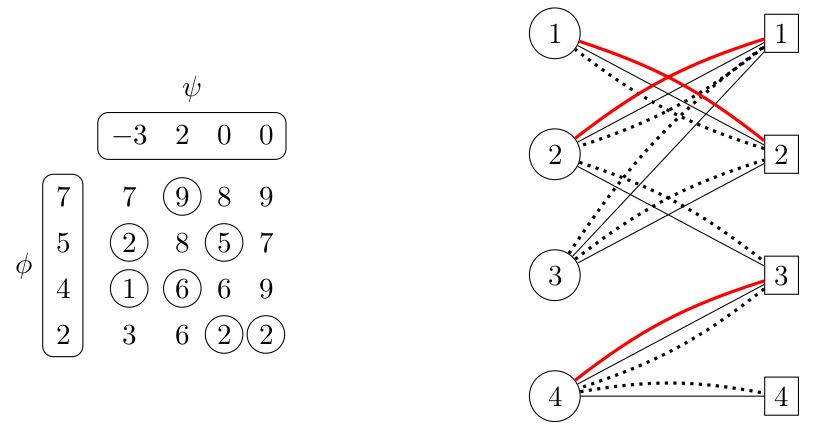
\includegraphics[scale=0.35]{z6.png}
	
\end{frame}

\begin{frame}
	\centering
	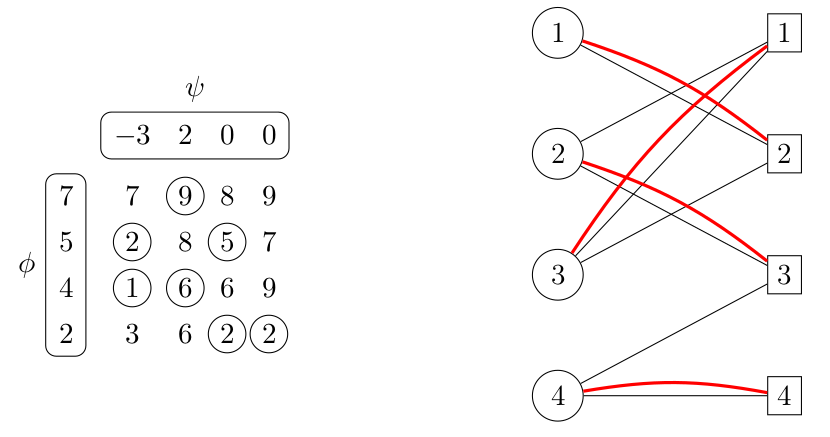
\includegraphics[scale=0.4]{z7.png}
	
\end{frame}

\begin{frame}
	\frametitle{Problème de production et de stockage en France}
	Modules pour l'algorithme Hongrois : \emph{'POT (Python Optimal Transport)', 'Munkres'
	'scipy.optimize.linear\_sum\_assignment', 'networkx.bipartite.minimum\_weight\_full\_matching'}

			\begin{minipage}[c]{1\linewidth}
		\begin{minipage}[c]{0.45\linewidth}\centering\begin{figure}
				\centering
				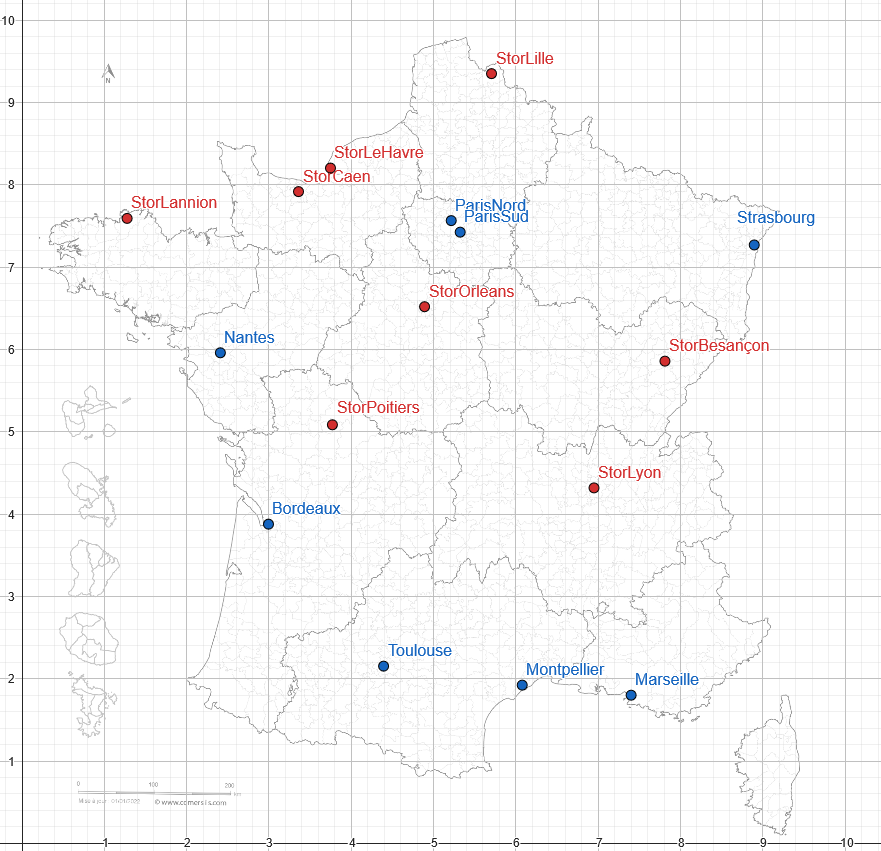
\includegraphics[scale= 0.25]{France.png}
		\end{figure}\end{minipage}\quad \quad 
		\begin{minipage}[c]{0.45\linewidth}\centering\begin{figure}
				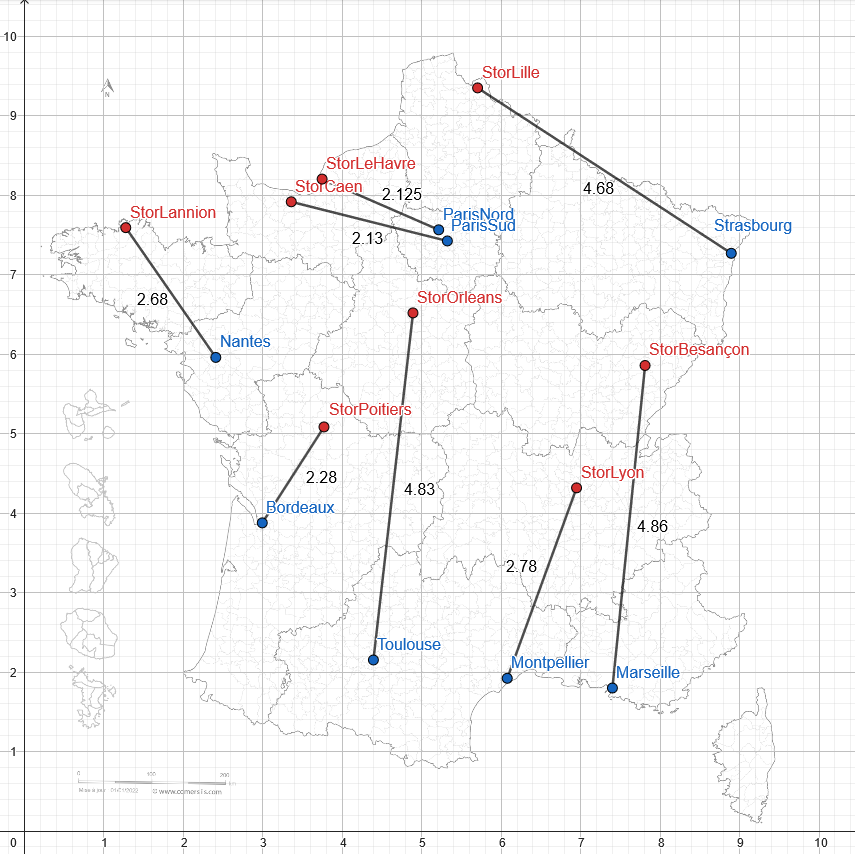
\includegraphics[scale= 0.25]{France1.png}		
				%\caption{Préparation du problème de transport optimal}
		\end{figure}\end{minipage}
	\end{minipage}
\end{frame}
\subsection{Applications à l'aide du module 'POT'}

\begin{frame}
	\frametitle{Transport optimal dans le plan}
		\begin{minipage}[t]{1\linewidth}
		\begin{minipage}{0.4\linewidth}\centering\begin{figure}
				\centering
				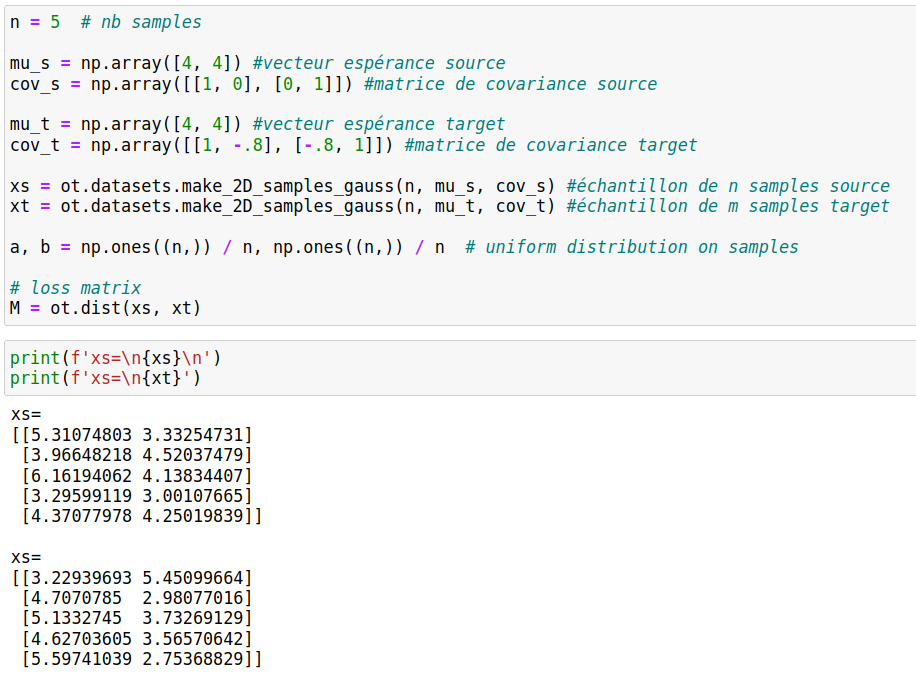
\includegraphics[scale= 0.34]{a1.png}
		\end{figure}\end{minipage}\quad \quad 
		\begin{minipage}{0.43\linewidth}\centering\begin{figure}
				\hfill\\[4cm]
				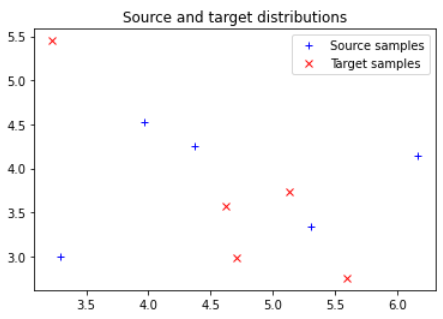
\includegraphics[scale= 0.36]{a2.png}		
				%\caption{Préparation du problème de transport optimal}
		\end{figure}\end{minipage}
	\end{minipage}
\end{frame}


\begin{frame}
	\begin{minipage}[t]{1\linewidth}
		\begin{minipage}{0.4\linewidth}\centering\begin{figure}
				\centering
				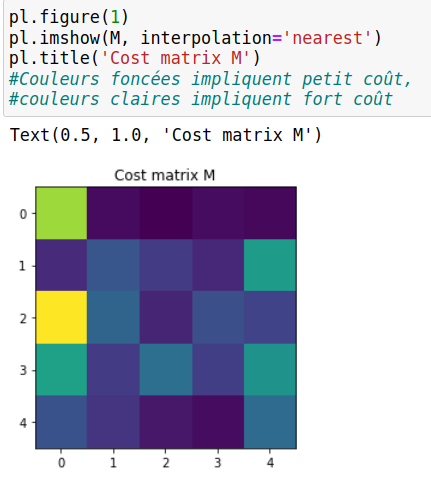
\includegraphics[scale= 0.5]{a4.png}
		\end{figure}\end{minipage}\quad \  
		\begin{minipage}{0.43\linewidth}\centering\begin{figure}
				\hfill\\[3cm]
				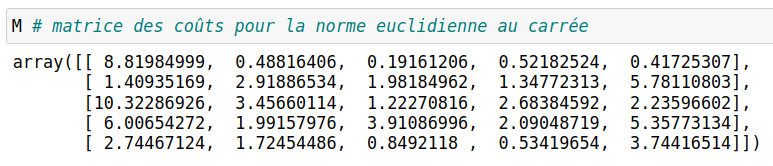
\includegraphics[scale= 0.25]{a3.png}		
				%\caption{Préparation du problème de transport optimal}
		\end{figure}\end{minipage}
	\end{minipage}
\end{frame}



\begin{frame}
		\centering
		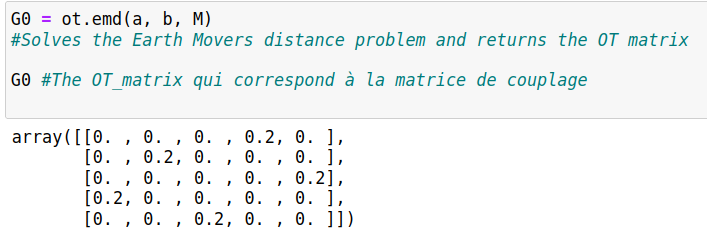
\includegraphics[scale= 0.45]{a7.png}
		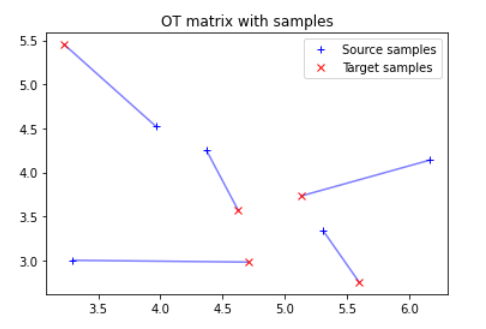
\includegraphics[scale= 0.45]{a5.png}
\end{frame}
\begin{frame}
	\frametitle{Transfert de couleurs entre deux images}
	
					\begin{minipage}[t]{1\linewidth}
			\begin{minipage}{0.4\linewidth}\centering\begin{figure}
					\centering
					\includegraphics[scale=0.14]{b3.jpg}
			\end{figure}\end{minipage}\hfil \quad \quad
			\begin{minipage}{0.43\linewidth}\centering\begin{figure}
					\centering
					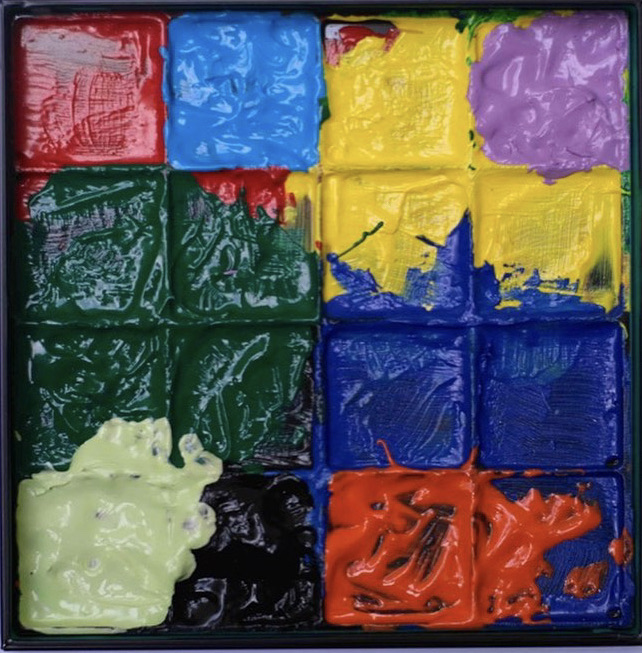
\includegraphics[scale=0.257]{b0.jpg}		
			\end{figure}\end{minipage}
		\end{minipage}
\end{frame}


\begin{frame}
	
	\centering
	
	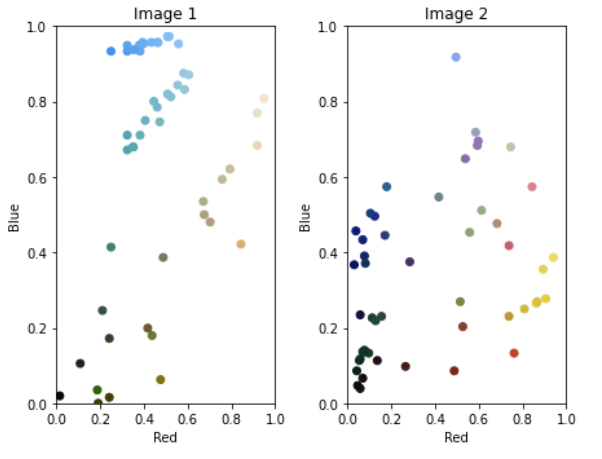
\includegraphics[scale= 0.65]{b32.png}
\end{frame}

\begin{frame}
	
	\begin{minipage}[t]{1\linewidth}\centering
	\begin{minipage}{0.4\linewidth}\centering\begin{figure}
	\centering
	\includegraphics[scale=0.12]{b3.jpg}
	\end{figure}\end{minipage} \quad \quad 
	\begin{minipage}{0.41\linewidth}\centering\begin{figure}
	\centering
	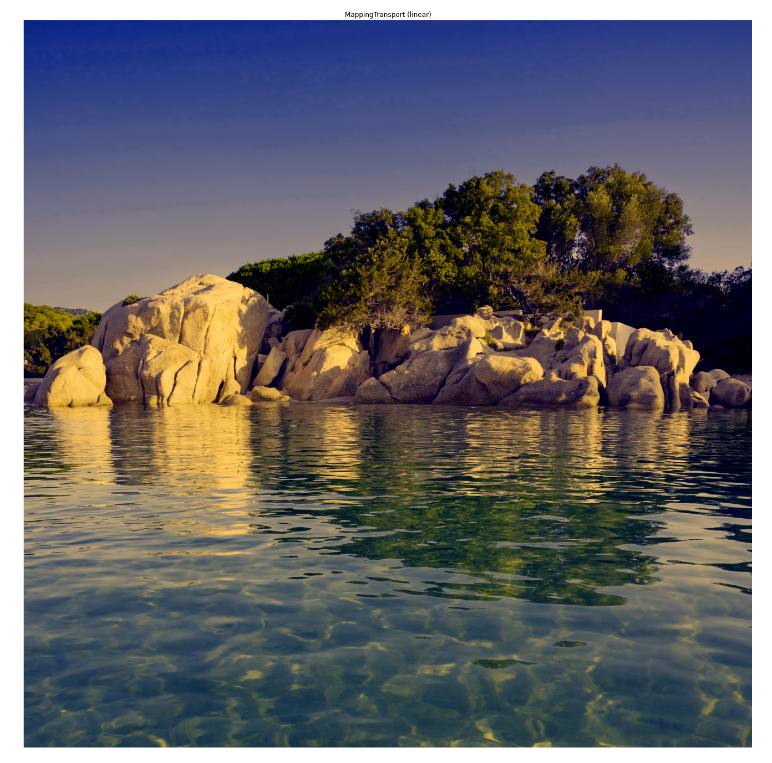
\includegraphics[scale=0.27]{b34.png}	
	\end{figure}\end{minipage}
	\end{minipage}
	
	
\end{frame}

\begin{frame}
	\frametitle{Modélisation du problème par Monge}\hfill\\[-0.8cm]
Peut-on construire une application $T : \R^2 \to \R^2$ transportant $\mu$ sur $\nu$ sous une certaine contrainte et avec un coût minimal ?\\ Autrement dit : comment transporter les points bleus sur les points
rouges avec un coût de transport minimal ? 


	
\end{frame}

\begin{frame}
	\frametitle{Modélisation du problème par Monge}\hfill\\[-0.8cm]

	Il y a plusieurs manières de transporter la "masse uniforme" bleue sur la "masse uniforme" rouge. Vous pouvez utiliser une translation, une symétrie ou encore une rotation. Les coûts associés à ces transporteurs pour la distance euclidienne varient. Comment choisir le meilleur transporteur ? 
	Ici la translation et la symétrie sont les transporteurs optimaux, il n'y a pas toujours unicité de la solution pour le problème de transport optimal. 
	
	
\end{frame}


\begin{frame}

	\begin{itemize}
		\item Soit $\displaystyle\mu = \sum_{i=1}^{n}\alpha_i\delta_{\{x_i\}}$ une mesure de probabilité source. 
		\item Soit $\displaystyle \nu = \sum_{i=1}^{m}\beta_i\delta_{\{y_i\}}$ une mesure de probabilité cible.
	\end{itemize}
	
\end{frame}

\begin{frame}
	
Voici le résultat obtenu pour le problème de transport optimal vu précédemment. Nous avons modélisé les points bleus et les points rouges à l'aide de deux familles de vecteurs Gaussiens avec des paramètres distincts. Le couplage entre les points s'effectue via un script Python qui utilise le module "POT: Python Optimal Transport". 


\end{frame}


\begin{frame}

La modélisation du problème de transport optimal proposée par Gaspard Monge trouve ses limites dans la division de la masse. Une application transport est déterministe, tout antécédent à une unique image par un transporteur T. Nous pouvons transporter les points bleus sources sur l'unique point rouge cible. En revanche le problème inverse ne trouve pas de solution au sens de Monge. Il est impossible d'envoyer le point rouge à quatre endroits différents.  
	
	
\end{frame}
\end{document}








